\section{Geometry Variations}

\begin{figure} 
\centering
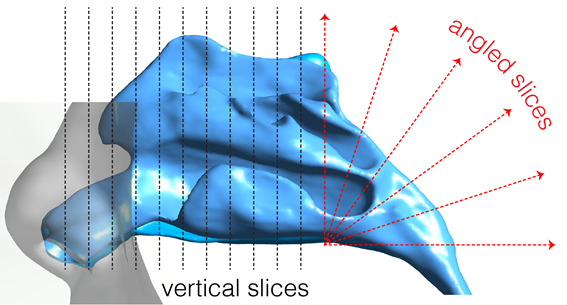
\includegraphics[width=0.7\textwidth]{slicesSchematic}
\caption{Representation of the slicing method used for sampling data across the sagittal axis throughout this thesis} 
\label{fig:Slices}
\end{figure}

One-hundred cross-sectional slices were taken from the nostrils tip to the nasopharynx. From nostrils tip to choanae, vertical slices were made, while angled slices were made in the nasopharynx until the slice became horizontal (Figure \ref{fig:Slices}).

\begin{figure} 
  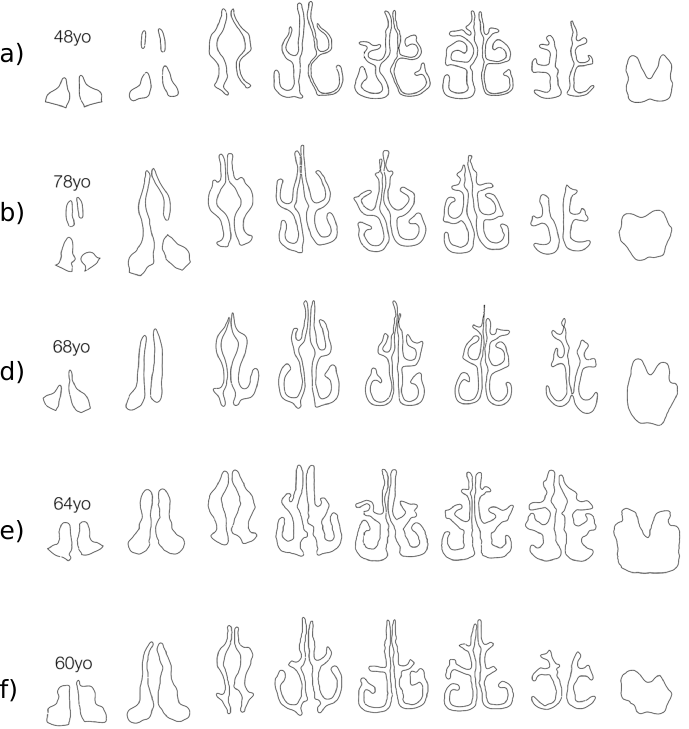
\includegraphics[width=\textwidth]{Silhouettes}
  \caption{silhouettes of the cavities}
  \label{fig:sil}

\end{figure}
Figure \ref{fig:sil} shows 8 coronal slices taken at equidistant spacing across the sagittal axis between the anterior vestibule and the nasopharynx. We see the airway elongate vertically which increases the perimeter but maintaining a relatively constant surface area. This area to perimeter ratio has been cited as an important factor in the development of fluid flow in the nasal cavity. The thinner cavities also tend to exhibit higher wall shear stress. This is because of the steeper velocity gradients, which create stress through the viscosity of air, near the wall. This narrowness is also likely to influence heat and vapour transfer in the cavities; when the cavities are narrower there is less distance for the heat and vapour to travel from the wall to saturate the incoming air, and so it is likely to saturate the airflow more comprehensively. The variation in cavity thickness between the cavities can also be clearly observed in this figure.

\begin{figure}
  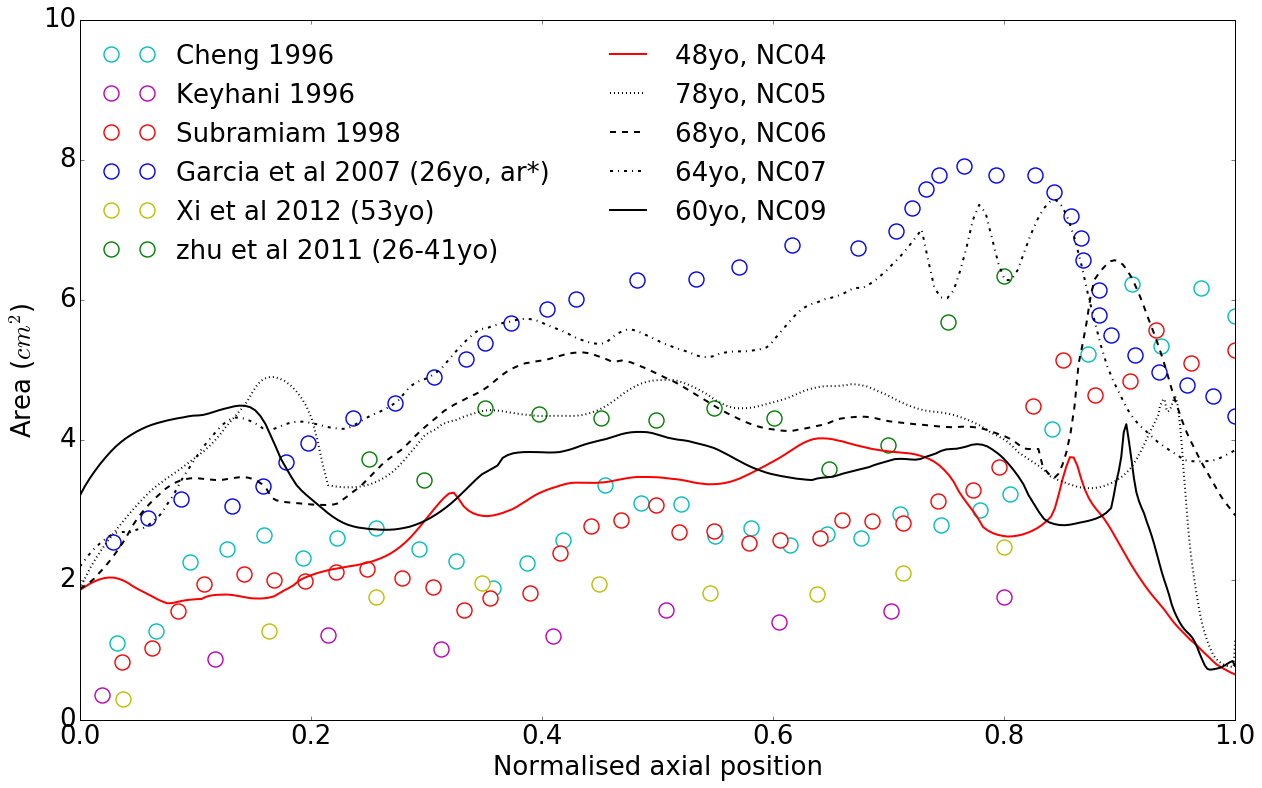
\includegraphics[width=\textwidth]{Areavsdistance}
  \caption{area versus distance across the four nasal cavities with a series of examples from the literature}
  \label{fig:area}
\end{figure}

Figure \ref{fig:area} shows the cross sectional area as a function of normalised distance along the sagittal axis. The distance has been normalised between the entrance to the nostrils and the end of the nasopharynx. A sample of cavities from the pre-existing literature has also been included for comparison. A significant variation can be seen in the average cross sectional area of the models presented in this paper; This variation is most pronounced towards the rear of the cavities. None of the models show quite the same volume as the atrophic rhinitis model, also shown here as Garcia prior to the nasopharynx, although the 64yo is close. The general shape of the curve is reasonably similar for the various models in this paper, with notable exceptions in the Nasopharynx of the 64yo cavity and a larger spike in the vestibule region of the 78yo. Observations from Figure 3 can be compared with the cross sectional silhouettes from Figure 2, for a clearer understanding of the variations in geometry between the 4 models presented here. The range of cross-sectional areas allows us to observe the relationship between various fluid mechanical properties of the cavity and cavity volume/cross-sectional area.

\begin{table}
  \begin{tabular}{p{0.125\textwidth}p{0.1\textwidth}p{0.1\textwidth}p{0.1\textwidth}p{0.1\textwidth}p{0.1\textwidth}p{0.11\textwidth}p{0.13\textwidth}}
 & \textbf{48yo} & \textbf{78yo} & \textbf{68yo} & \textbf{64yo} & \textbf{60yo} &\textbf{Xi et al. \cite{Xi2012}} & \textbf{Garcia et al.\cite{Garcia2007}} \\
\cline{2-8}
\textbf{Turbinal region} & 18.54 & 22.78 & 24.62 & 30.722 & 16.73 & 12.63 & 33.66\\
\textbf{Naso-pharynx}  & 3.84 & 5.40 & 12.80 & 20.09 & 4.57 & 16.33 & 10.60\\
\textbf{Vestibule} & 3.10 & 4.15 & 2.81 & 4.21 & 7.39 & 5.50 & 2.41\\
\textbf{Total} & 25.48 & 32.33 & 40.23 & 55.07 & 28.69 & 34.43 & 47.77 \\
\hline
\end{tabular}
\caption{ sectional volume, according to sections as seen in Figure \ref{fig:regions} ($ cm^3 $)}\label{tab:secvol}
  \begin{tabular}{p{0.125\textwidth}p{0.1\textwidth}p{0.1\textwidth}p{0.1\textwidth}p{0.1\textwidth}p{0.1\textwidth}p{0.11\textwidth}p{0.13\textwidth}}
 & \textbf{48yo} & \textbf{78yo} & \textbf{68yo} & \textbf{64yo} &\textbf{60yo}& \textbf{Xi et al.} & \textbf{Garcia et al.}\\
 \cline{2-8}
\textbf{Turbinal region} & 170.92 & 174.07& 190.44 & 163.44 & 138.80 & 112.59 & 133.50\footnote{includes vestibule} \\
\textbf{Naso-pharynx} & 12.20 & 12.80 & 25.23 & 40.42 & 11.37 & 40.93 & 31.46\\
\textbf{vestibule} & 15.71 & 17.37 & 12.45 & 17.92 & 46.96 & 35.58 &  -\\
\textbf{total} & 198.82 & 204.25 & 228.11 & 221.79 & 197.192 & 189.10 & 164.96\\
\hline
\end{tabular}
\caption{sectional surface area, according to sections shown in Figure \ref{fig:regions}($ cm^2 $)}\label{tab:secsa}
  \begin{tabular}{p{0.125\textwidth}p{0.1\textwidth}p{0.1\textwidth}p{0.1\textwidth}p{0.1\textwidth}p{0.1\textwidth}p{0.11\textwidth}p{0.13\textwidth}}
& \textbf{48yo}  & \textbf{78yo} & \textbf{68yo} & \textbf{64yo} & \textbf{60yo} & \textbf{Xi et al.} & \textbf{Garcia et al.}\\
 \cline{2-8}
\textbf{Turbinal region} & 0.434 & 0.52 & 0.52 & 0.75 & 0.48 & 0.45 & 1.11\\
\textbf{Naso-pharynx} & 1.26 & 1.69 & 2.03 & 1.99 & 1.61 & 1.60 & 1.35\\
\textbf{vestibule} & 0.79 & 0.96 & 0.90 & 0.94 & 0.63 & 0.62 &  - \\
\textbf{total} & 0.51 & 0.63 & 0.71 & 0.99 & 0.58 & 0.72 & 1.13 \\
\hline
\end{tabular}
\caption{Effective diameter $d_{eff} = \frac{4v}{a} (cm) $}\label{tab:deff}

  \begin{tabular}{p{0.125\textwidth}p{0.1\textwidth}p{0.1\textwidth}p{0.1\textwidth}p{0.1\textwidth}p{0.1\textwidth}p{0.11\textwidth}p{0.13\textwidth}}
& \textbf{48yo}  & \textbf{78yo} & \textbf{68yo} & \textbf{64yo} & \textbf{60yo} & \textbf{Xi et al.} & \textbf{Garcia et al.}\\
 \cline{2-8}
 \textbf{MCA}&1.665&3.0174&1.80&4.14&2.7&Unknown&3.04
\end{tabular}
 \caption{Minimal axial cross sectional area $(cm^2)$}\label{tab:mca}
\end{table}

\begin{figure}
\centering
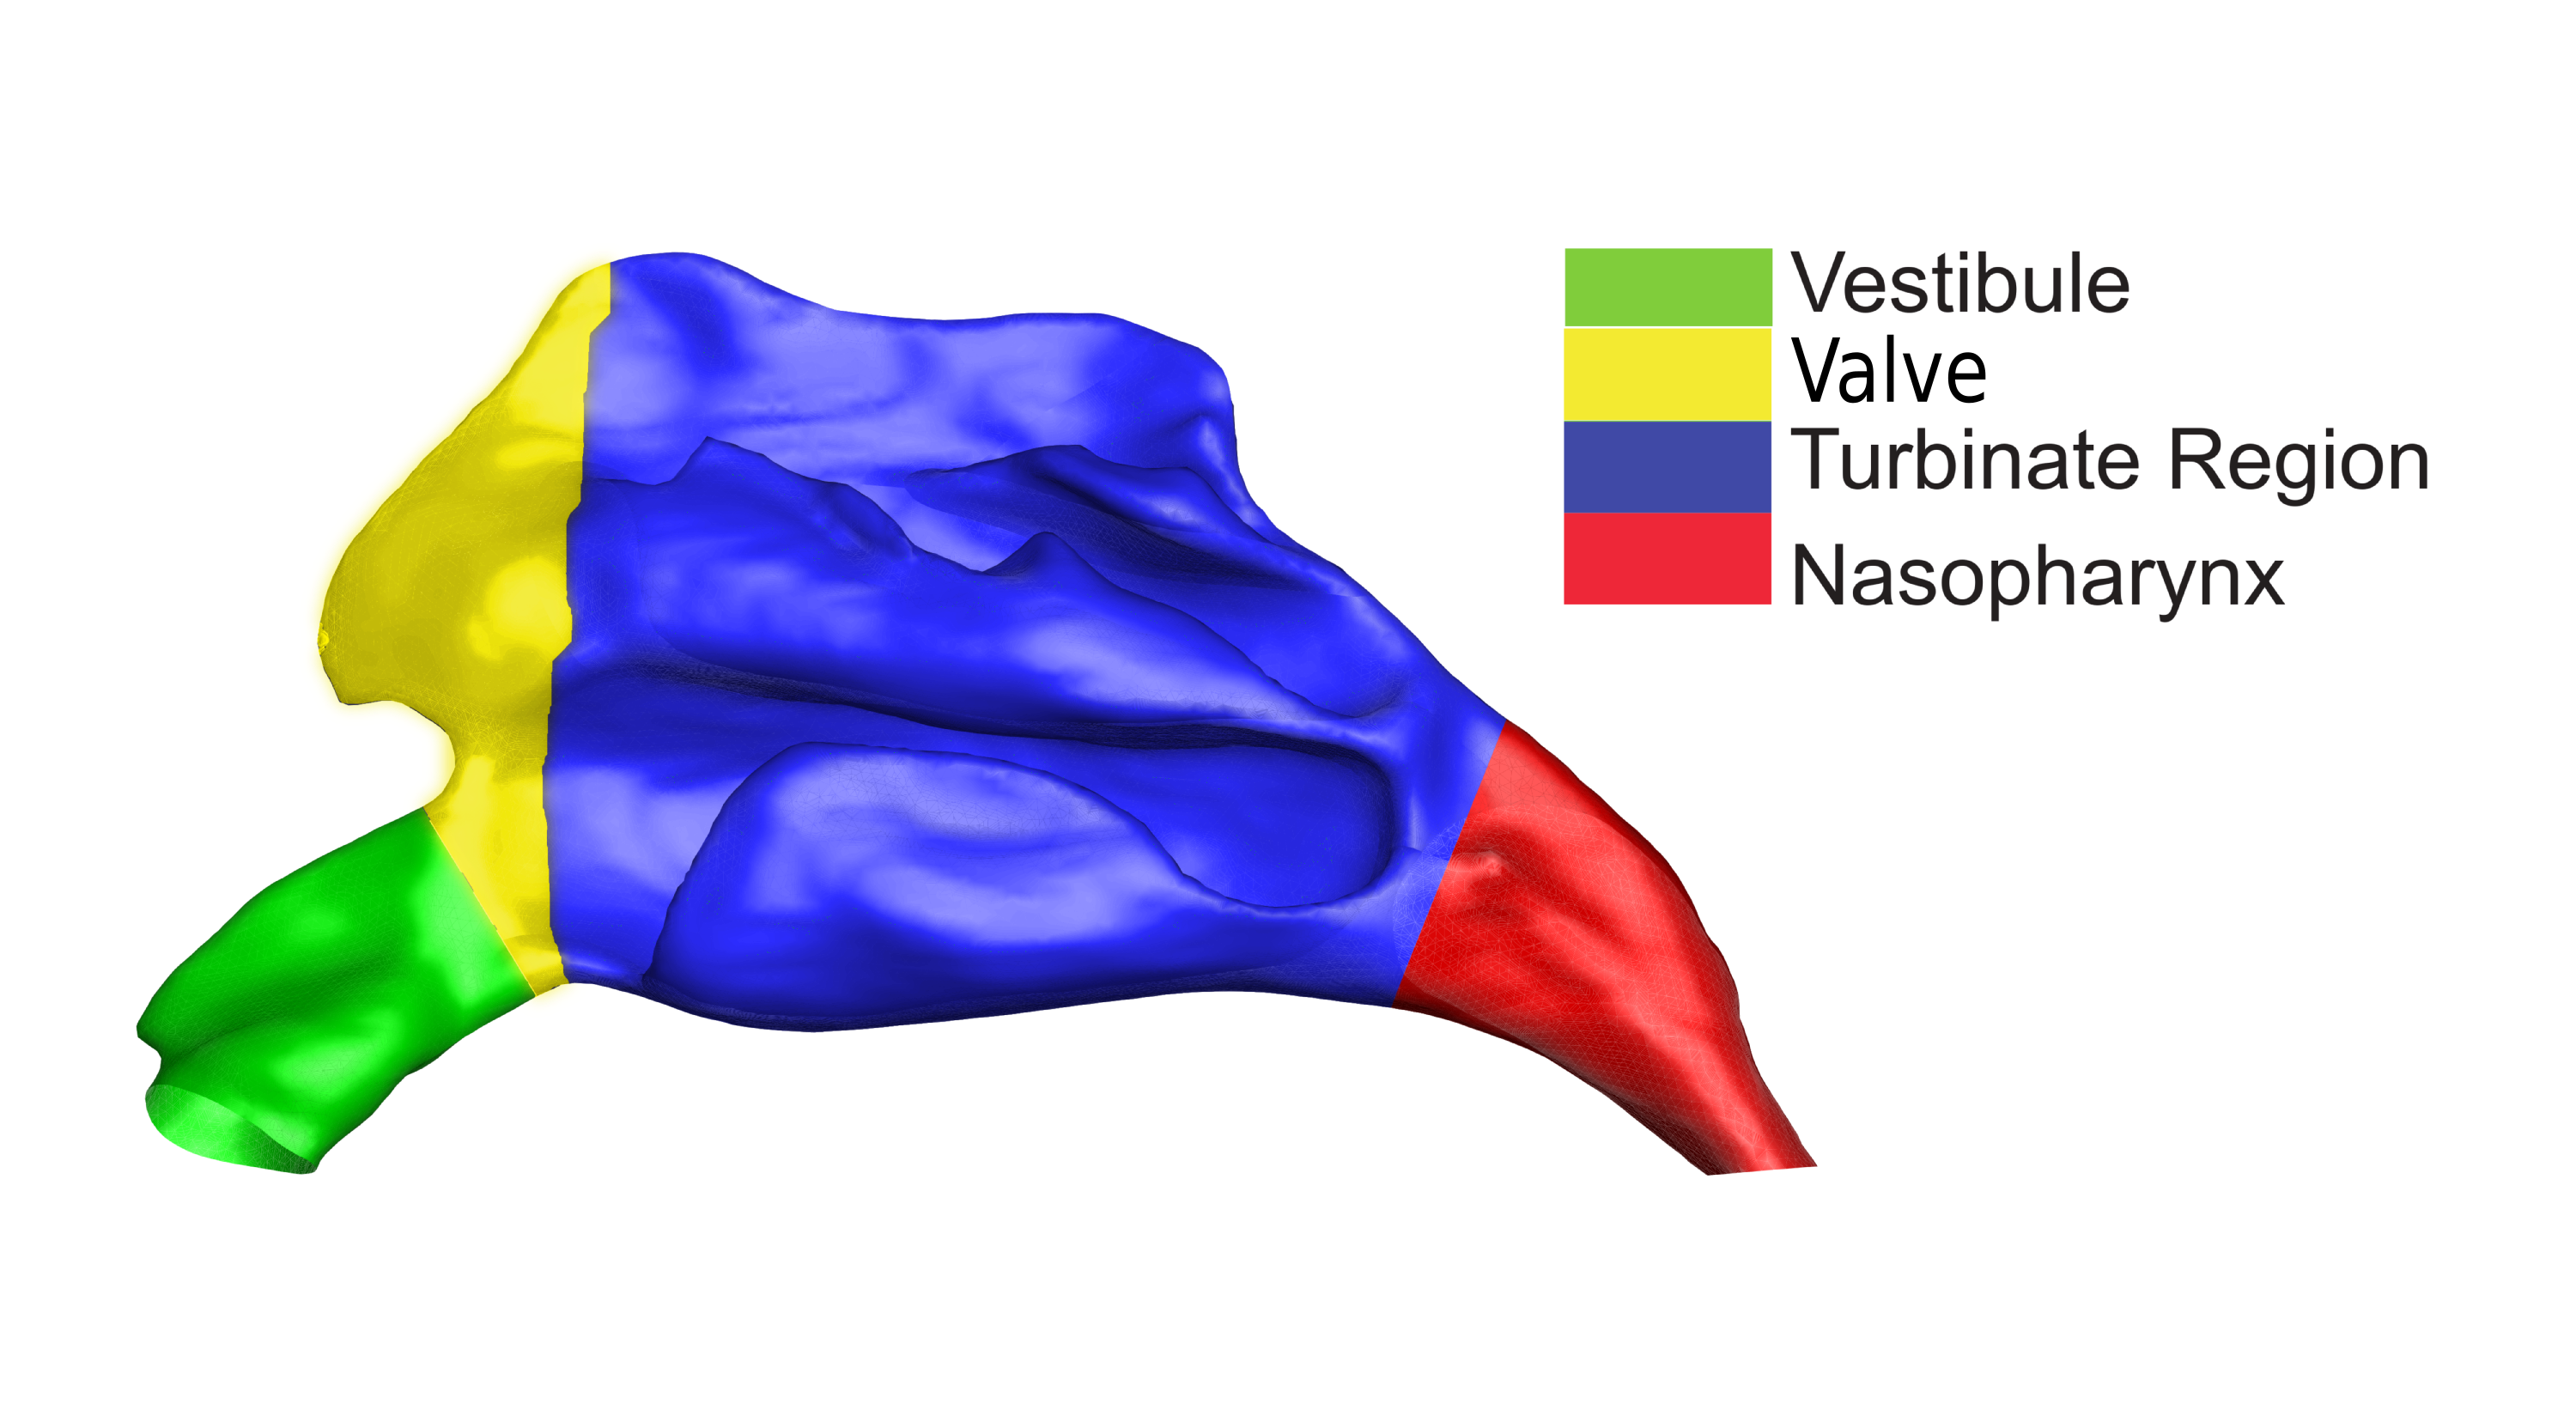
\includegraphics[width=0.7\textwidth]{regions}
\caption{Colour coded display of the regional divisions used in tables \ref{tab:secvol}, \ref{tab:secsa}, \ref{tab:deff}} 
\label{fig:regions}
\end{figure} 

Table \ref{tab:secvol} - \ref{tab:deff} shows the variation of the volume, surface area and effective diameter respectively, in comparison with models from the literature. The volumes of the four models presented in this paper varied significantly. The largest discrepancies were noted in the pharynx and turbinate regions, with a less marked discrepancy in the vestibular region. The 48 – yo is showing greater volume than that seen in the atrophic rhinitis patient from \cite{Garcia2007}. The surface area of the atrophic rhinitis model is also significantly lower, to the extent that the effective diameter, shown in Table \ref{tab:deff}, is larger than the models presented in this paper.

Minimal cross sectional area, shown in Table \ref{tab:mca}, is significant to flow across the cavity\cite{Lindemann2008}. Here the atrophic rhinitis model shows larger minimal cross sectional area than any of those found in the models presented here, although it is quite close to that of the 64yo.

The circularity shape factor (a dimensionless quantity used in image analysis) was used to quantify the cross-sectional shape (Figure \ref{fig:Circ}). The circularity, $f_o$ , (also known as the isoperimetric quotient), is the ratio of cross-sectional area bounded by a closed curve, to its perimeter defined as, 

$ f_o = \frac{4 \pi A}{P^2} $

At the nostril inlet, the circularity ranges from 0.18-0.30 and this reduces to a value of approximately = 0.035 (except the 64yo model). It then increases rapidly towards 1 where the two nasal chambers merge and form a single conduit in the form of the nasopharynx.







\begin{figure}
\centering
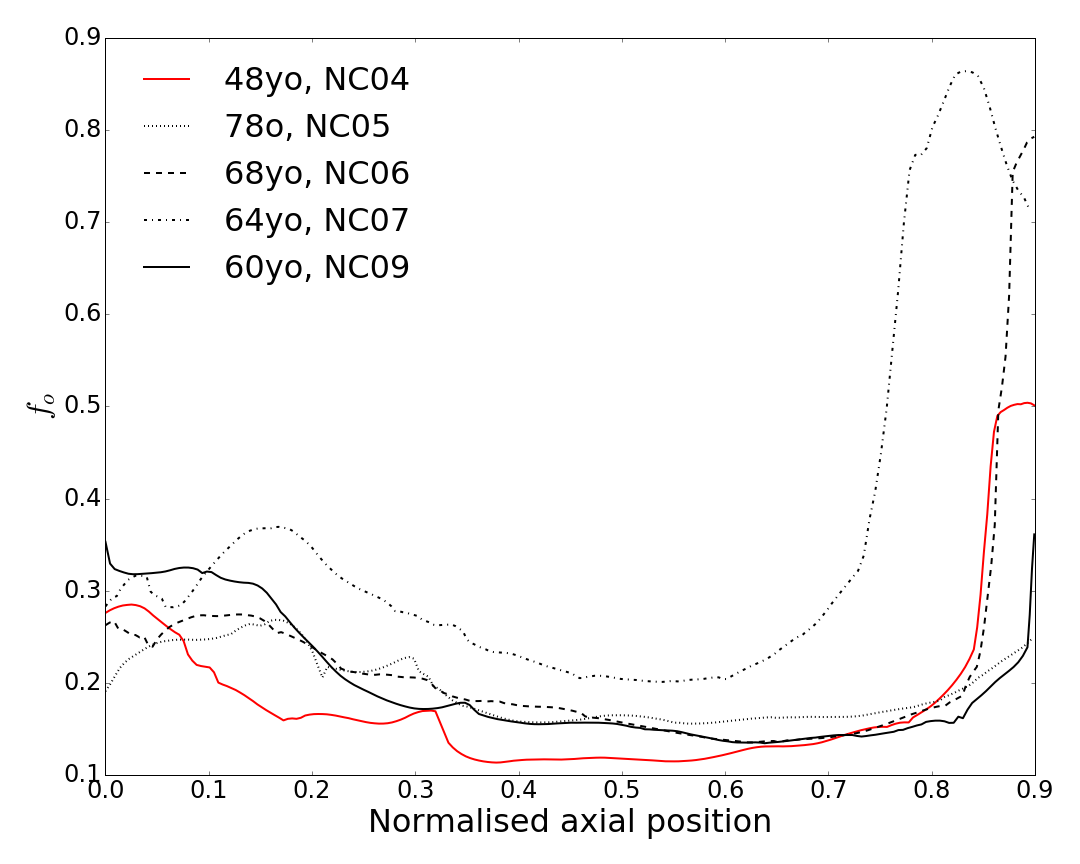
\includegraphics[width=1\textwidth]{circularity}
\caption{area to perimeter ratio variation with normalised length of the nasal cavity from the nostril inlet to the nasopharynx. This length for each model is: 48yo – 8.97cm; 60yo – 9.26cm; 64yo – 9.60cm; 68yo – 9.31cm; 78yo – 8.45cm}
\label{fig:Circ}
\end{figure}

\section{Pressure Drop}

The pressure drops across the nasal cavities can also be seen in Figure \ref{fig:stpr} to vary in relation to the volume of the nasal cavity. This is in contrast to the experimental findings of \cite{Lindemann2008, Edelstein1996, WhanKim2007}, who’s studies using rhinomanometry showed no significant decrease in pressure across the cavity to accompany the recorded variation in volume. The cause of this discrepancy is unclear. Here the pressure drop is primarily seen across the valve region. Here the nasopharynx has been excluded from the domain; the significant pressure drop across the nasopharynx was inversely proportional to the cross sectional areas of the respective nasal cavities

The pressure drops can be seen in Figure \ref{tab:pvv} to decrease in relation to the volume of the cavity. This fits well with the findings of previous experimental studies looking at pressure drops across nasal cavity models, as can be seen from the comparison with results from \cite{Garcia2007} and \cite{Kelly2004}, both displayed in figure \ref{tab:pvv}.

  \begin{table} 
    \centering
  \pgfplotstableset{
  every head row/.style={before row=\toprule,after row=\midrule},
  every last row/.style={after row=\bottomrule}}

  \pgfplotstabletypeset[
      fixed zerofill,
      precision=2,
      display columns/0/.style={string type},
      col sep=comma]{tables/prvsflow.txt}
  \caption{Variation of pressure drop with flow rate (m/s)}
  \label{tab:pvv}
\end{table}

\begin{figure} 
  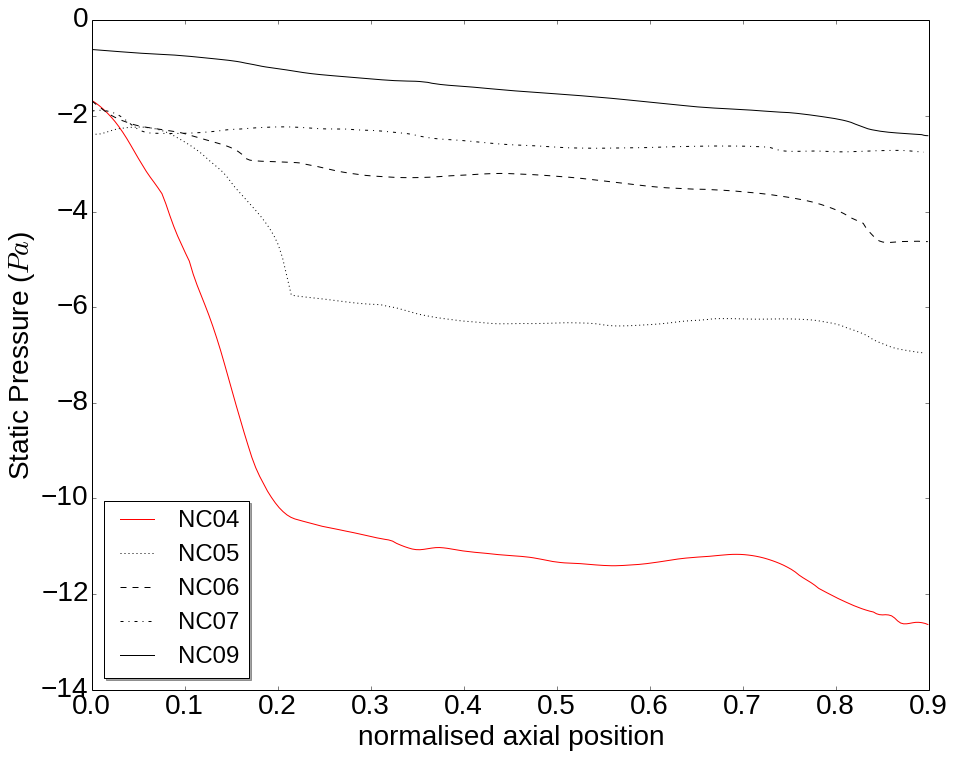
\includegraphics[width=\textwidth]{statpres}
  \caption{area versus distance across the four nasal cavities with a series of examples from the literature}
  \label{fig:stpr}
\end{figure}

\section{Wall Shear Stress and velocity}
Figure \ref{fig:vsl} shows flow streamlines through the left and right nasal chambers with the chamber’s wall shear stress. In all the models flow acceleration and high wall shear stresses were consistently found in the region between the nasal vestibule entrance (anterior) and before the middle nasal passage. We also note that there is a preference for the streamlines to pass through the mid-height of the nasal chambers. A small fraction reached the olfactory region, and some inferiorly along the floor of the chambers. The highest wall shear stress values were found in the 48yo, 60yo, and 78yo models which are also the models with the smaller cross-sectional area profiles (from Figure \ref{fig:area}), and corresponds to the highest velocity magnitudes produced by the streamlines in the models. Wall shear stress contours viewed from the top and lateral left-chamber side of all nasal models are shown in Figure \ref{fig:wcont}. By using the same colour scale the results show directly the disparity between nasal models.

Figure \ref{fig:wcont} shows the wall shear stress across the five models presented in this paper. The valve region can be seen to be a region of particularly high wall shear across all the models. Also note that the locations of high wall shear vary significantly in the more voluminous cavities


From Figure \ref{fig:wax}, Wall shear stress can be seen to be more pronounced in general in the more voluminous models such as the 48yo, and in particular this effect is exaggerated in the valve region. Here the wall shear stress is mapped rom the nostrils to the entrance to the nasopharynx. The nasopharynx showed more pronounced variations, in particular the 48yo showed a significant spike in wall shear stress in the nasopharynx, which is to be expected because of its lower cross sectional area. Note that the sagittal distribution of wall shear stress is much more even in the larger cavities.  The valve region - considered of particular significance to the development of flow features within the nasal cavity \cite{Lindemann2008} – shows significant variation in wall shear stress concentration, with the 64yo and 60yo presenting a very even distribution of wall shear stress, in contrast to the 48yo or 78yo which show wall shear more pronounced around the opening from the vestibule. Similar variations can also be seen in the distribution within the turbinal region (Figure \ref{fig:wcont}). 

Cross-sections at the internal nasal valve, and turbinate region were taken for each model and its velocity contour presented in Figure \ref{fig:wcs}. We traced the perimeter of each cross-section starting from its apex and follow down in a counter-clockwise direction. For the nasal valve cross-section in all models, we found that the surface proportion was distributed almost evenly between the lateral and septum walls, since its partition occurred at 0.5. For the turbinate region, this value was 0.7 meaning that 70\% of the perimeter resides along the lateral side and 30\% of the perimeter is along the septum wall. For the 48yo model we labelled three peaks for the nasal valve slices (r1, r2, and l1) to help identify the locations on the cross-section itself. 

Wall shear stress peaks occurred close to the regions of maximum velocities in the contours. Superiorly, where the velocity is very low, the wall shear stress is nearly zero. These peaks and troughs correlate well with the contour slices and is consistent for all models.

\begin{figure} 
  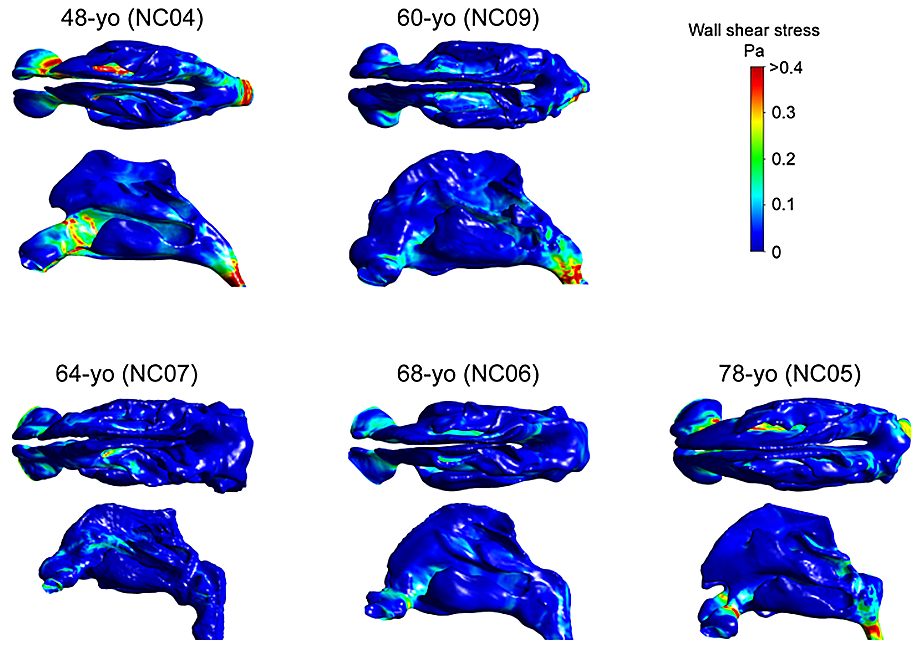
\includegraphics[width=\textwidth]{wsscont}
  \caption{Direct comparison of WSS surface contours between all models}
    \label{fig:wcont}
\end{figure}

\begin{figure} 
  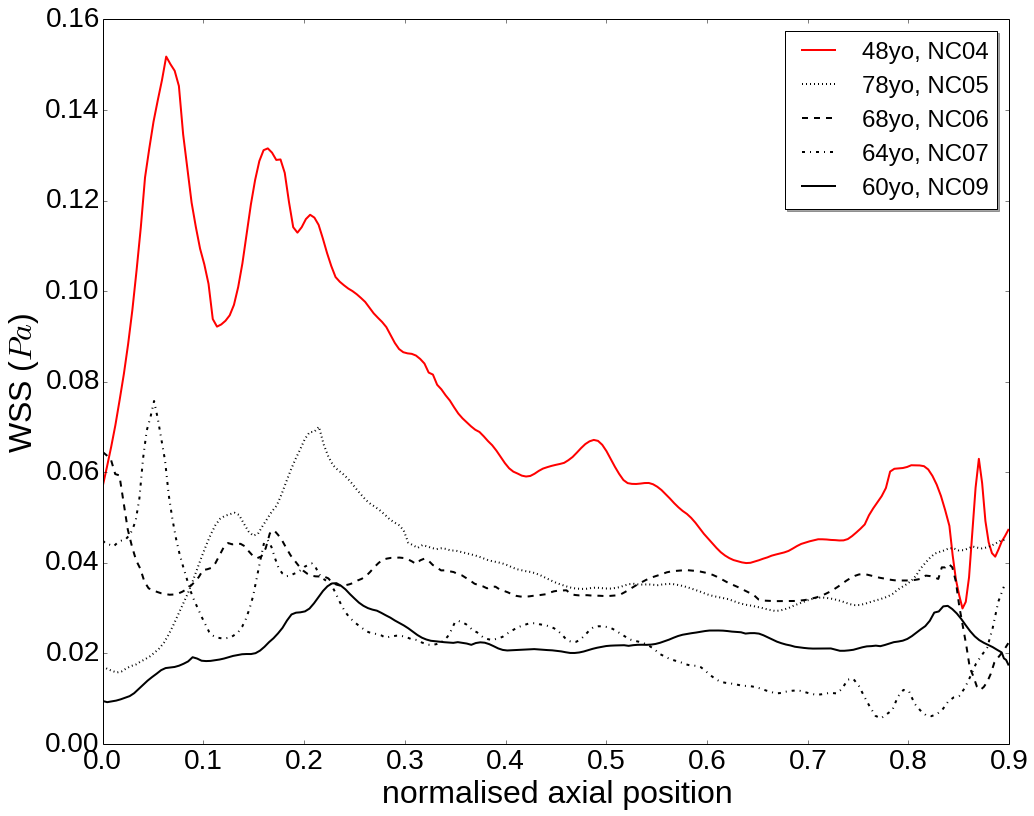
\includegraphics[width=\textwidth]{axialwss}
  \caption{coronal area weighted average of wall shear stress plotted as a function of distance from the entrance to the cavity across the saggital axis}
  \label{fig:wax}
\end{figure}

\begin{figure} 
  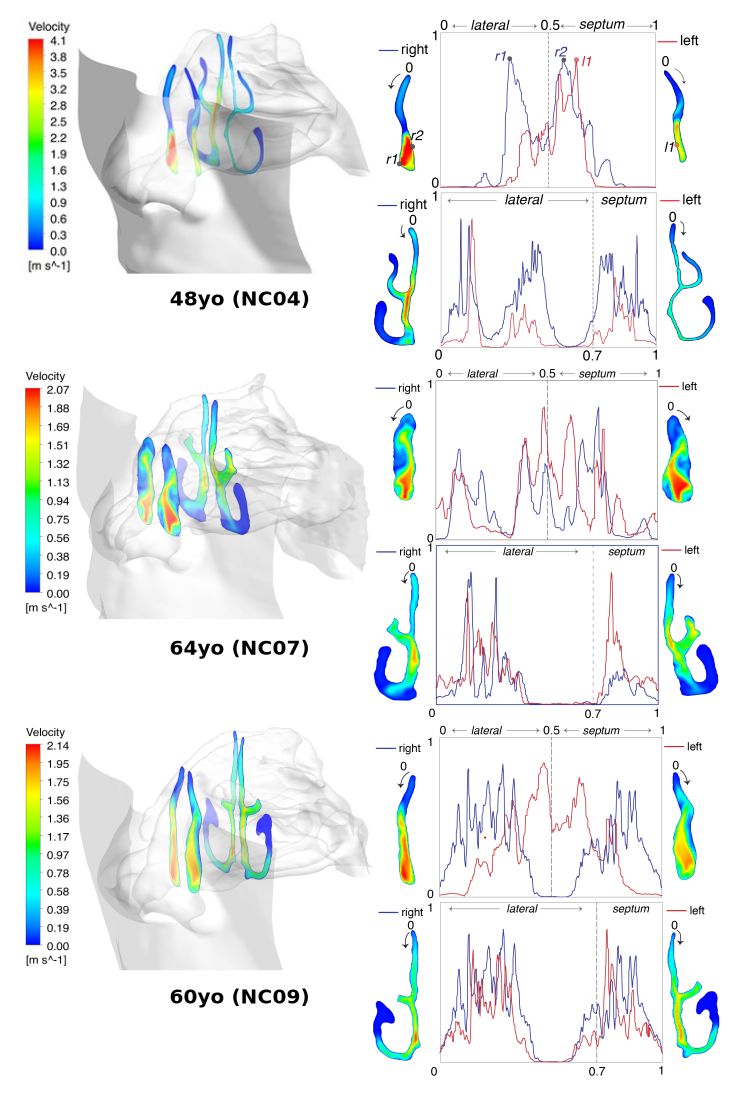
\includegraphics[width=\textwidth]{wsscs/wsscs1}
  \label{fig:wcs}
\end{figure}

\begin{figure} 
  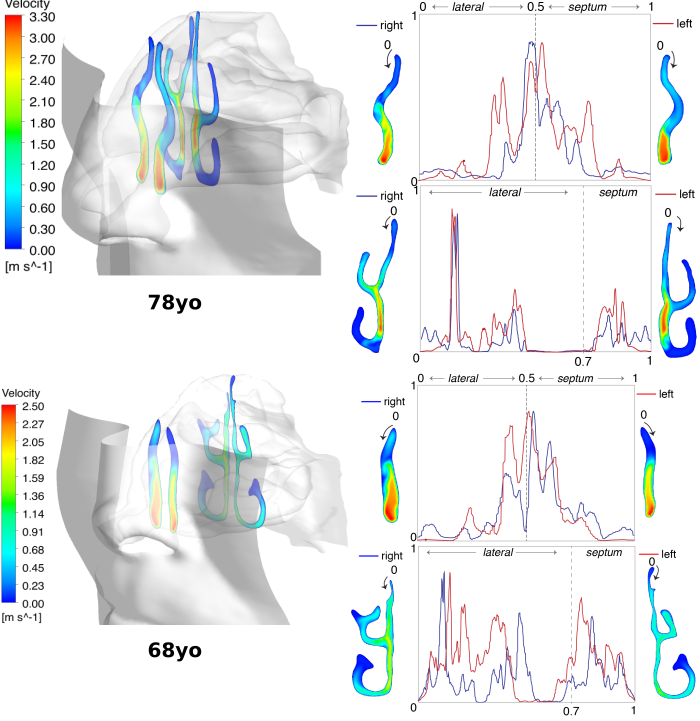
\includegraphics[width=\textwidth]{wsscs/wsscs2}
  \caption{Velocity contours and wall shear stress values along the perimeter outlines of two cross-sections. The x-axis is the perimeter distance starting from the top apex of each cross-section slice, and moves along the perimeter laterally. One full tracing around the perimeter is defined as 1.0. The dashed line represents the floor of the cross-section opposing its apex, and for the nasal valve, the halfway point \(0.5\), while for the turbinate cross-section it is 0.7. The y-axis represents normalized wall shear stress \(0 - 1\).}
  \label{fig:wcs}
\end{figure}

\begin{figure} 
  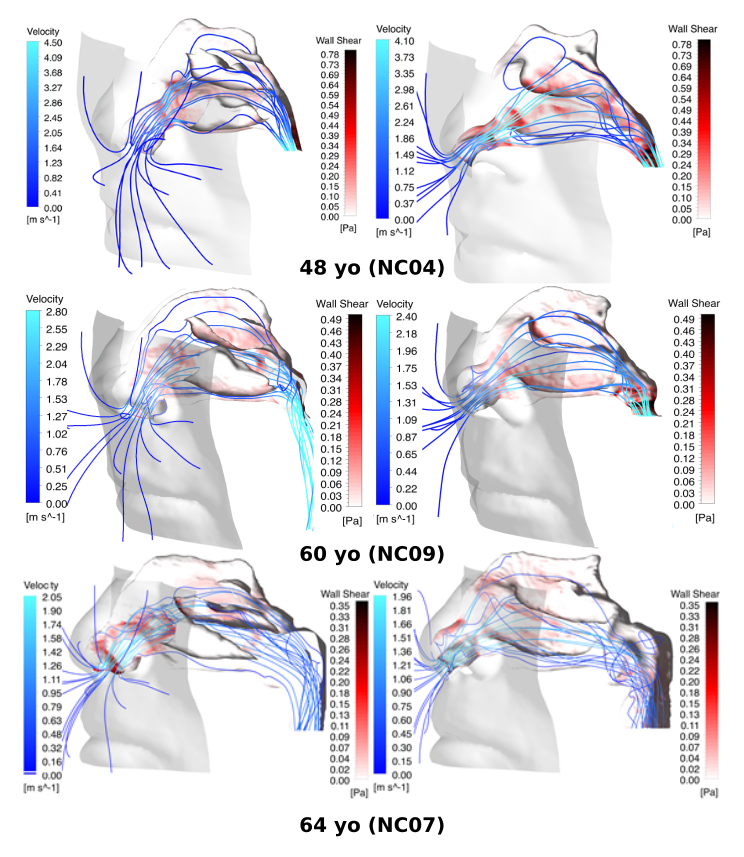
\includegraphics[width=\textwidth]{streamlines/sl1}
  \end{figure}

\begin{figure} 
  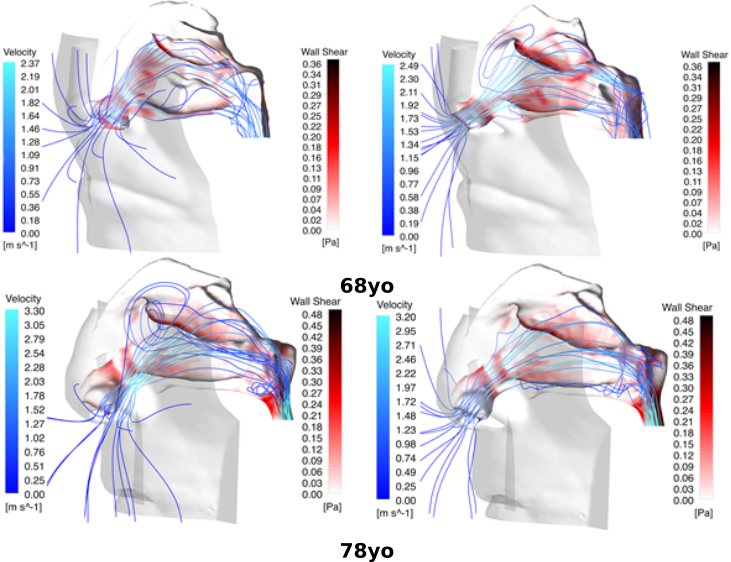
\includegraphics[width=\textwidth]{streamlines/sl2}
  \caption{Flow streamlines (coloured in blue) passing through the left and right chambers of the nasal cavity. Each chamber’s wall shear stress is shown (coloured in red).}
  \label{fig:vsl}
\end{figure}

 
\section{Heat and Vapour Transfer}

Some variation in the heat and vapour transfer efficacy can be seen between the models presented in this thesis. Note the higher than average figures for temperature and h2o mass fraction in the valve area of the 78yo. In general the more voluminous models exhibit lower humidity and temperature (Figures \ref{fig:h2o} and \ref{fig:Temp}). The data from the atrophic rhinitis study by Garcia et al \cite{Garcia2007}; the humidity and temperature distribution in this model seem to be lower in proportion to the increased voluminousness of this model (see figure \ref{fig:area}).

\begin{figure} 
  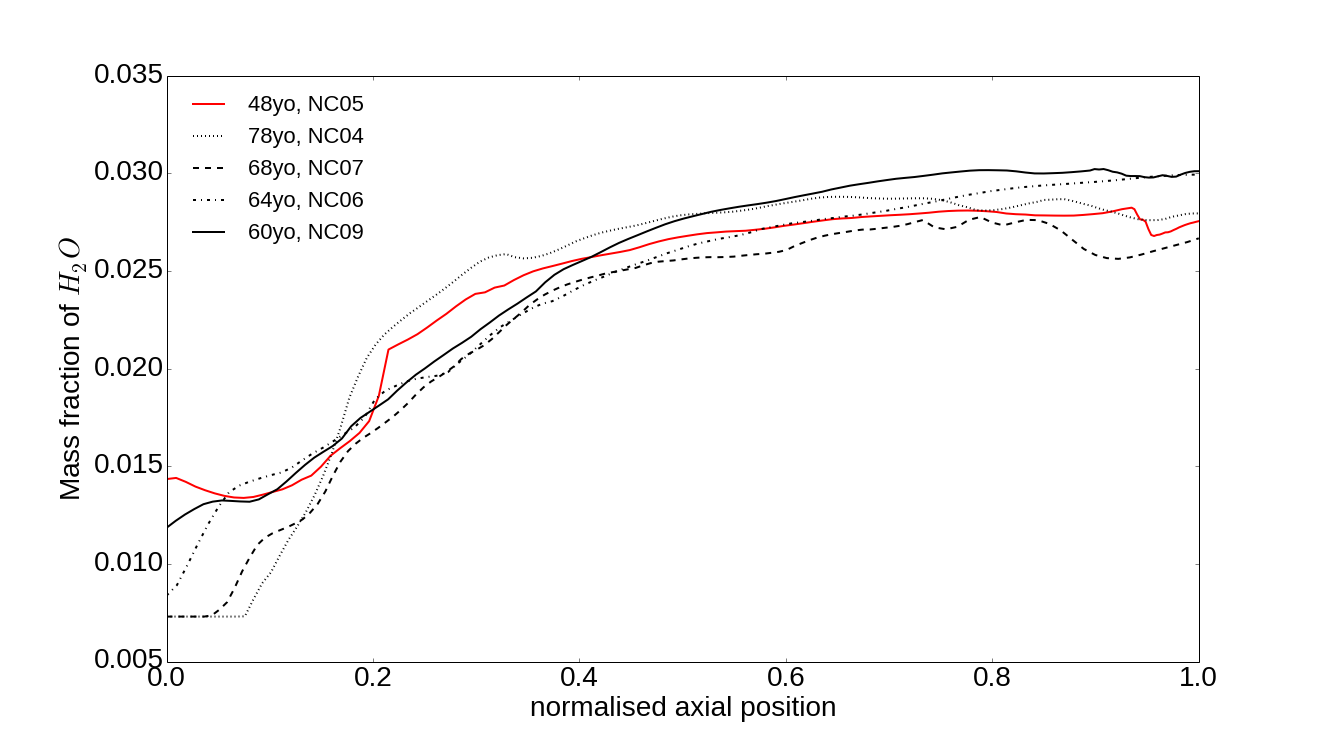
\includegraphics[width=\textwidth]{h2o}
  \caption{average mass fraction of h2o as a function of normalised saggital position}
  \label{fig:h2o}
\end{figure}


\begin{figure} 
  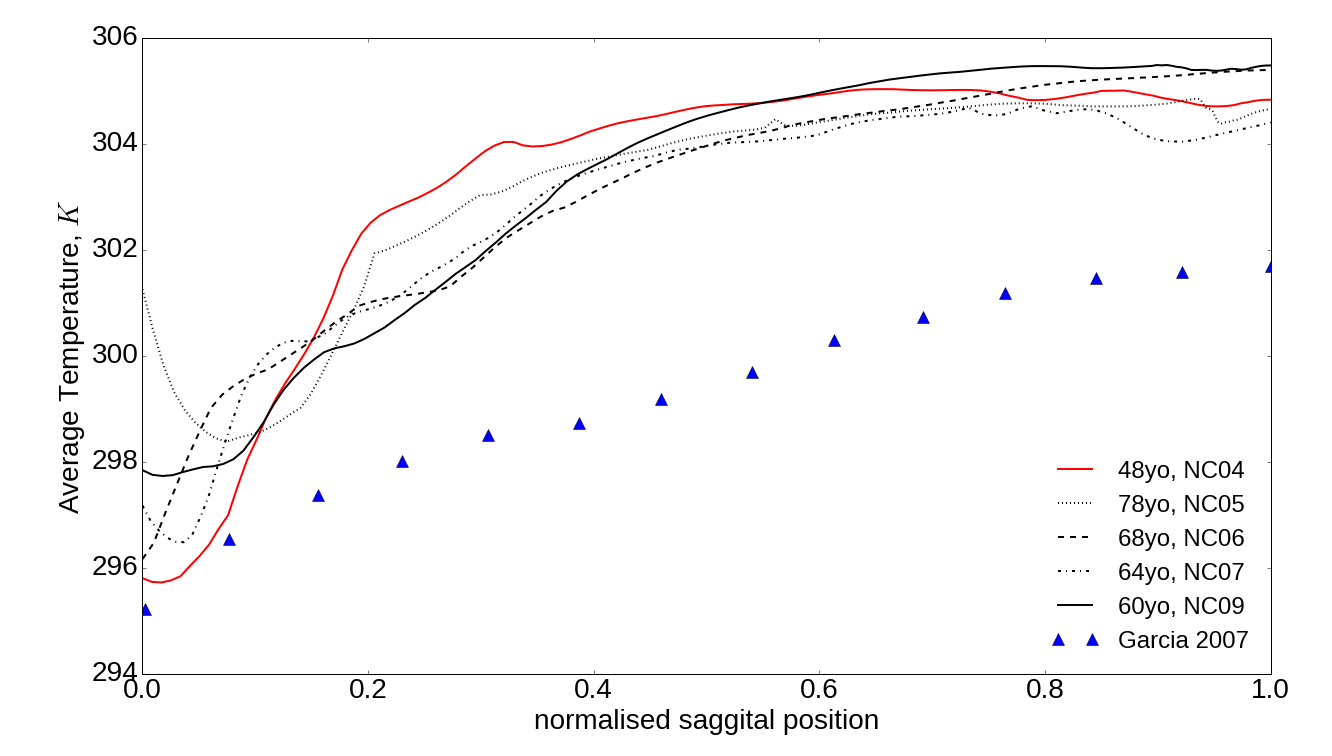
\includegraphics[width=\textwidth]{Temperature}
  \caption{average ambient temperature as a function of normalised saggital position}
  \label{fig:Temp}
\end{figure}
